\section{Sprint  Overview}
The development cycle that is being followed is a feature driven development.
The features and milestones were created at the beginning of the semester.
Sprint were handled in two week incriments and features were assigned to 
the sprints to be accomplished during the two weeks. The backlog consisted
of what was going to be accomplished in the coming weeks and what was not
completed in the last sprint. At the begining/end of each sprint, the 
developers would get together for a sprint planning/retrospective, to discuss
how to previous sprint went and how to handle the up coming one.


\section{Terminology and Acronyms}
% Provide a list of terms used in the document that warrant definition.  Consider 
% industry or domain specific terms and acronyms as well as system specific. 

\begin{itemize}
	\item Augmented Reality (AR): hardware and software that, together, superimpose computer-generated images on a user's view of the real world. Often, this composite view may be interacted with. 

	\item Virtual Reality (VR): hardware and software that, together, create a computer-generated simulation of a three-dimensional image or environment. Often, this simulation may be interacted with. 

	\item Mixed Reality (MR): the overlap in domain space of augmented reality and virtual reality. 

	\item Microsoft HoloLens: portable and cordless augmented reality viewing device. 

	\item Meta 2: augmented reality viewing device that must be connected to a computer and power outlet. 

	\item Mira Prism: augmented reality viewing device that leverages a user's mobile device.

	\item Oculus Rift: virtual reality viewing device. 

    \item QR Code: machine readable matrix barcode optical label.
    
    \item Unity: video game engine used in creating HoloLens apps.

	\item Cloud: off-site computing and digital storage resources accessed via the internet. 

    \item Azure: Microsoft Cloud hosting feature

	\item .fbx: model file type that may be rendered by most AR devices on the market. 
\end{itemize}


\section{Sprint Schedule}
As stated above, sprints were two weeks long. Each sprint was designed to accomplish a milestone. 
Below is the schedule of the sprints and what was accomplished during those sprints.

\begin{itemize}
	\item 9/18/2017   - Define milestones and user stories

	\item 10/2/2017   - Base website created with file upload ability
	
	\item 10/16/2017  - Wireframes, Presentation 1 documents, standalone file conversion
	
	\item 10/30/2017  - File upload/download, file conversion integrated
	
	\item 11/13/2017  - QR code generation, standalone advanced file conversion 
	
	\item 11/27/2017  - File conversion integration, create users, Presentation 2 documents
	
	\item 12/04/2017  - Finish documentation, second semester prep
	
	\item 12/13/2017  - MVP delivered to sponsor
	
	\item 04/27/2017  - Final product delivered to sponsor.
\end{itemize}

\section{Timeline}
Below is the timeline of accomplished milestones.

\begin{figure}[H]
\begin{center}
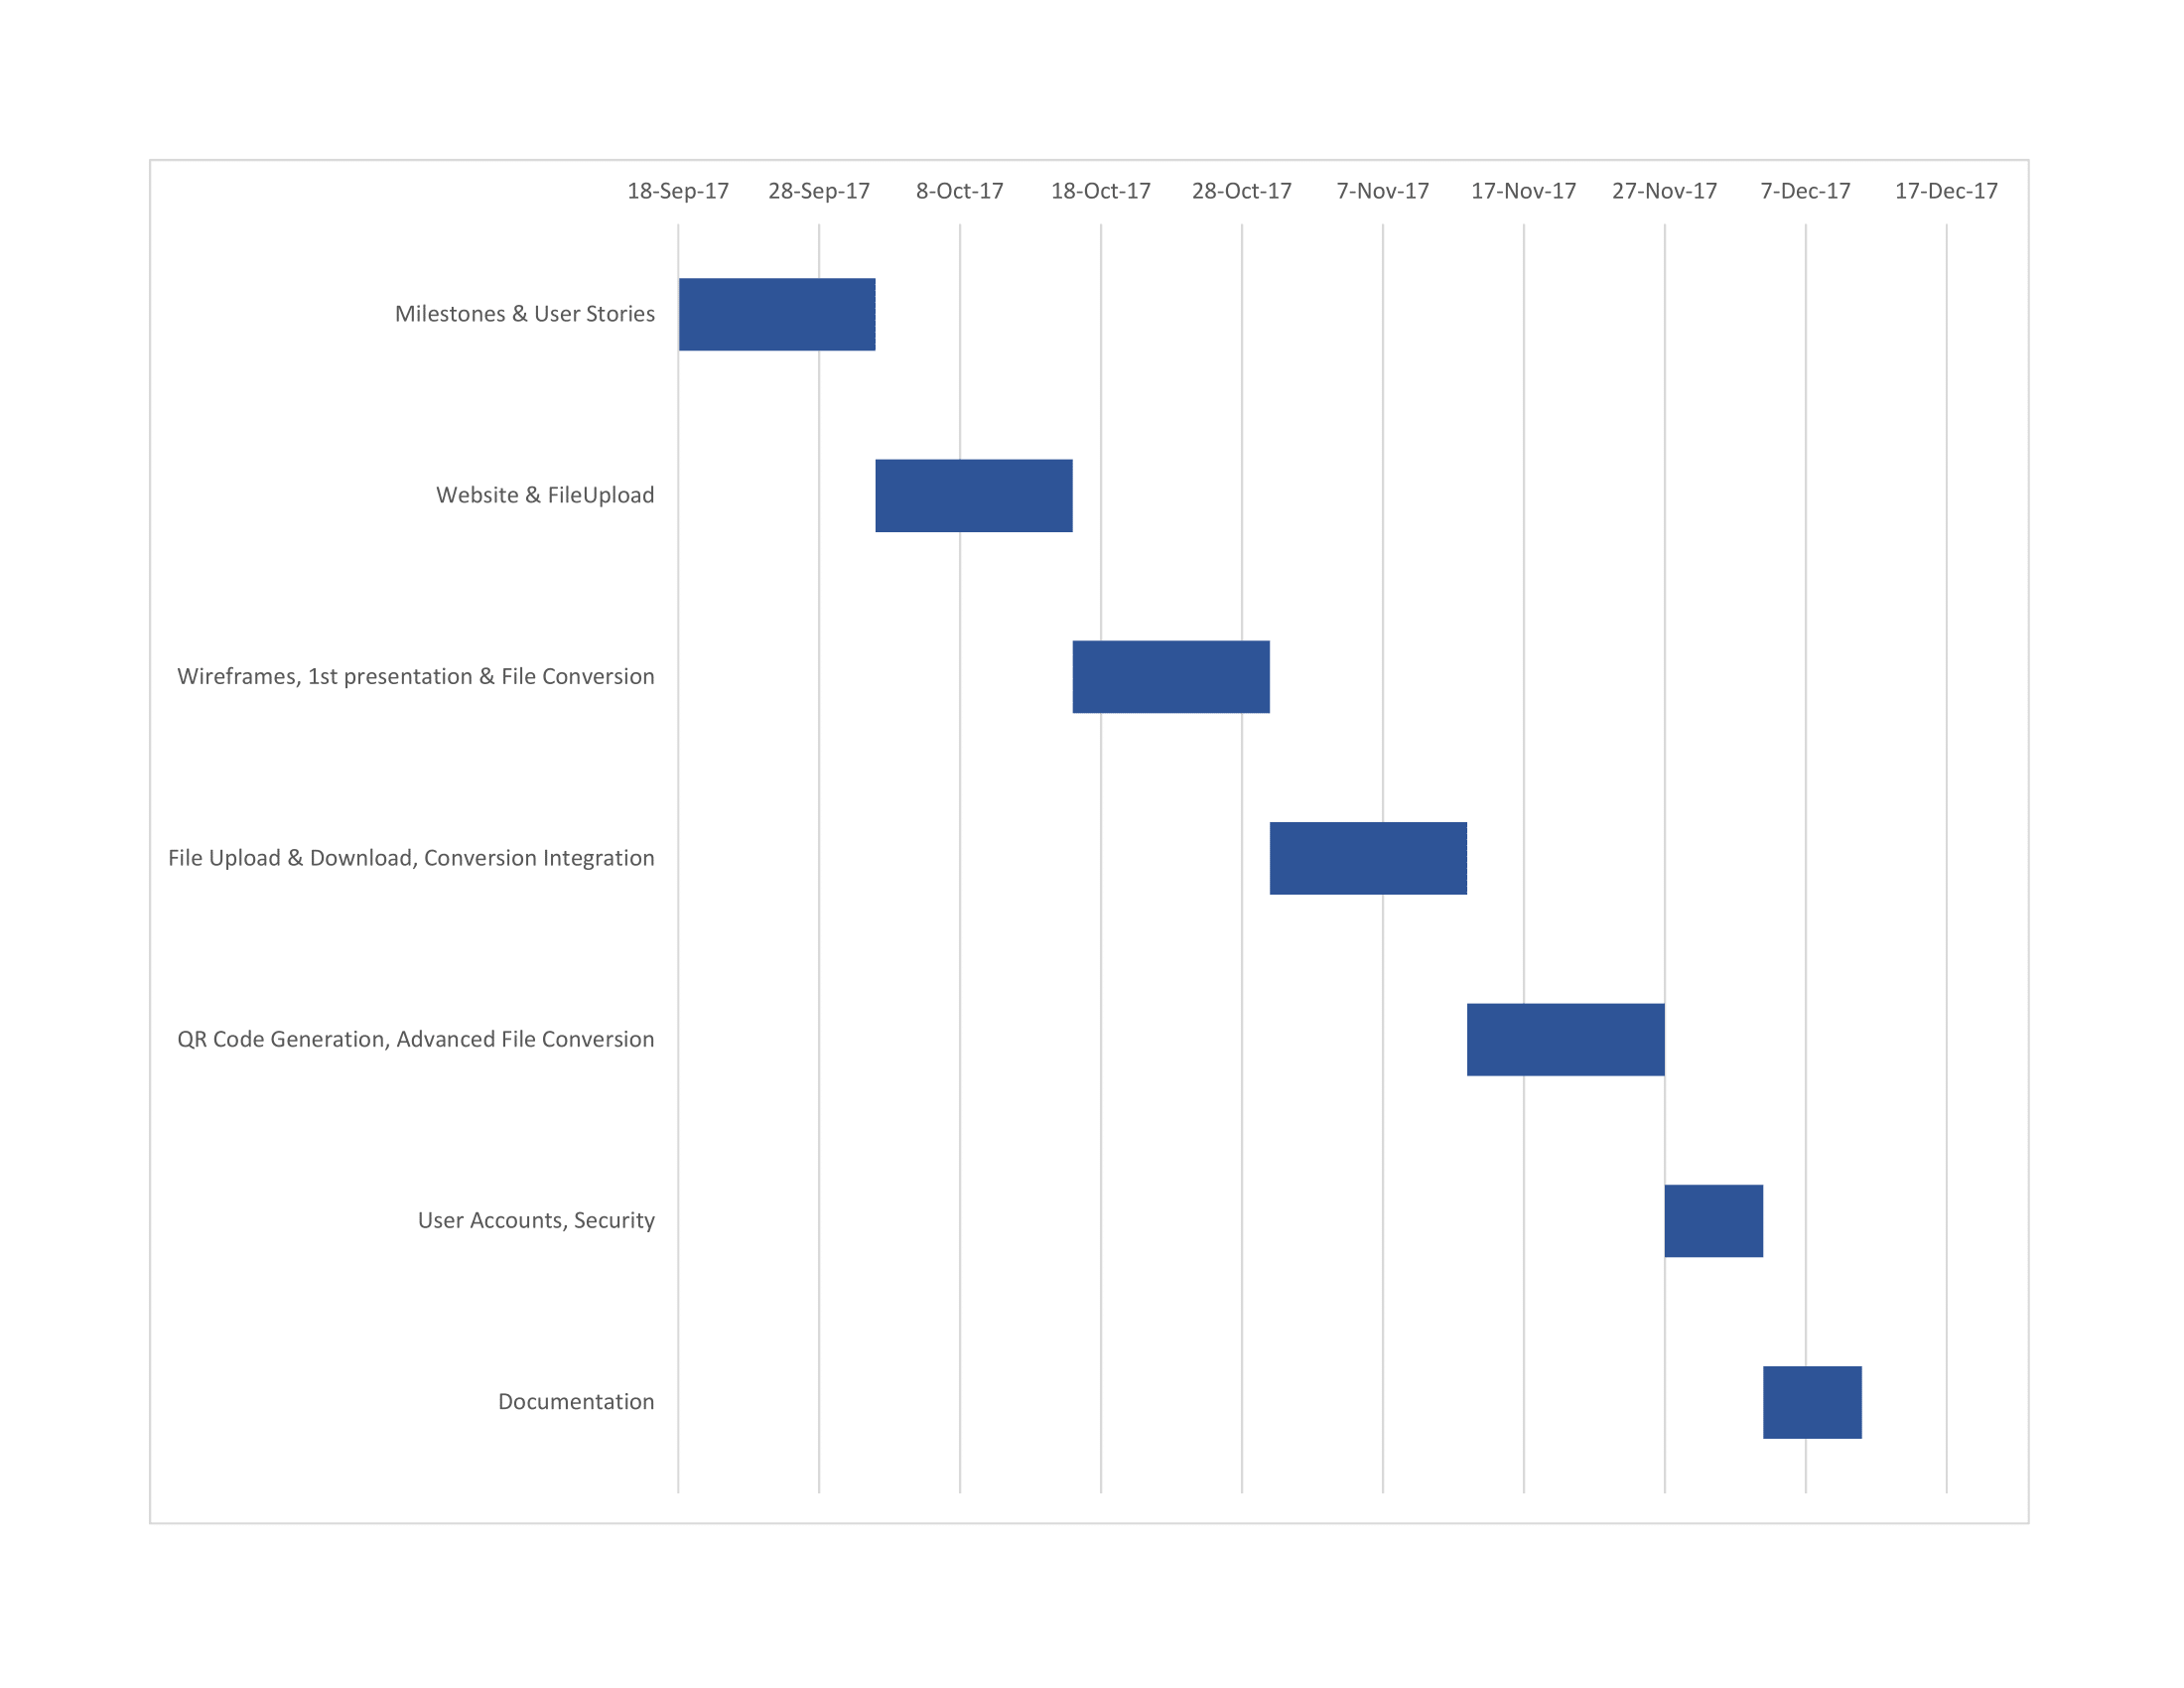
\includegraphics[width=1\textwidth]{./SprintGanattChart}
\end{center}
\caption{Sprint Timeline}
\end{figure}
